\documentclass[twoside,11pt]{article}

% Any additional packages needed should be included after jmlr2e.
% Note that jmlr2e.sty includes epsfig, amssymb, natbib and graphicx,
% and defines many common macros, such as 'proof' and 'example'.
%
% It also sets the bibliographystyle to plainnat; for more information on
% natbib citation styles, see the natbib documentation, a copy of which
% is archived at http://www.jmlr.org/format/natbib.pdf

\usepackage{jmlr2e}
\usepackage{amsmath}
\usepackage{amssymb}
\usepackage{enumitem}
\usepackage{subcaption}
\usepackage{float}
\usepackage{cleveref}
\usepackage{hyperref}


% Definitions of handy macros can go here

\newcommand{\dataset}{{\cal D}}
\newcommand{\fracpartial}[2]{\frac{\partial #1}{\partial  #2}}

% Heading arguments are {volume}{year}{pages}{submitted}{published}{author-full-names}

%\jmlrheading{1}{2000}{1-48}{4/00}{10/00}{Marina Meil\u{a} and Michael I. Jordan}

% Short headings should be running head and authors last names

%\ShortHeadings{Ensemble Methods for Robust Feature Selection}{Meil\u{a} and Jordan}
\firstpageno{1}

\begin{document}

\title{Ensemble Methods for Robust Feature Selection}
%TODO write C-SVM and not SVM
%TODO check if it is written that same weights are ranked random
\author{\name Benjamin Rabier \email benjamin.rabier@campus.tu-berlin.de \\
       \addr Neural Information Processing Group\\
       Technical University Berlin\\
       10623 Berlin, Germany
       \AND
       \name Alexander Goscinski \email a.goscinski@mail.tu-berlin.de \\
       \addr Neural Information Processing Group\\
       Technical University Berlin\\
       10623 Berlin, Germany}

\editor{No Editor}

\maketitle

\begin{abstract}%   <- trailing '%' for backward compatibility of .sty file
  Abstract
\end{abstract}

\begin{keywords}
  Ensemble Methods, Robust, 
\end{keywords}

\section{Introduction}

Feature selection is a method used in machine learning to find a small subset of features to build a more accurate, simpler and faster model. It is often used with high dimensional data. Moreover it allows domain experts to gain a better understanding of the data, by focusing on the selected subset. However, in domains such as biomedical applications subsequent analysis are costly. Thus not only the model performance but also the robustness of the feature selection method is important. Domain experts would prefer a more stable algorithm to have more confidence in the selected features. One approach for more robust results are ensemble methods.

Used in machine learning and statistics, ensemble methods combine multiple algorithms in order to obtain better performance. The bagging method for feature selection, which consists of using the same algorithm on multiple subsets, has already been studied in \cite{saeys2008}. The method improved the robustness of the feature selection algorithm considerably while the model performance is not significantly degraded in most cases. The purpose of this paper is to extend on these results and investigate the effect of ensemble methods further by combining different feature selection methods.

\section{Feature selection methods}
\label{sec:fs_methods}
Symmetrical Uncertainty (SU) \citep{press1996numerical} is an entropy based measurement. It is the normalized mutual information between the feature and the class. The mutual information measures the influence of the knowledge of the class on the feature value in terms of entropy and normalizes it. It is defined as follows:
\begin{equation}
  \label{eq:su}
  SU(F,C) = 2 \frac{H(F) - H(F|C)}{H(F) + H(C)} \textrm{, where } H(\cdot) \textrm{ is the entropy.}
\end{equation}
More details about mutual information can be found in \cite{paninski2003estimation}. 

The second feature selection is RELIEFF \citep{kononenko1997overcoming}. For each sample $x_i$ the k nearest neighboring samples, using the $L_1$ norm as metric, belonging to the same class $\{\textrm{Near-hit}_{i, j}\}_{j=1..k}$ and the ones of the opposite class $\{\textrm{Near-miss}_{i, j}\}_{j=1..k}$ are selected. Then the difference is taken to update the weight vector representing how well each feature distinguishes samples of the two classes, as can be seen in equation \ref{eq:relief}. In all the experiments k is set to 5, which empirically gives satisfactory results.
\begin{equation}
  \label{eq:relief}
  W_i = W_i - \frac{1}{k}\sum_{j=1}^{k}|x_i - \textrm{Near-hit}_{i,j}| + \frac{1}{k}\sum_{j=1}^{k} |x_i - \textrm{Near-miss}_{i,j}|
\end{equation}
The third feature selection method uses recursive feature elimination (RFE) with a linear C-SVM classifier \citep{guyon2002gene} to weight the features. 
The RFE method fits a classifier and ranks the feature according to their importance in the model. In the case of the C-SVM, it is based on the weight vector of the hyperplane. More precisely after obtaining the solution for the primal problem of the C-SVM in equation \ref{eq:svm_primal}, the ranking coefficients $c_i$ for the features are then calculated by squaring the weights $c_i = w_i^2$.
\begin{alignat}{-1}
     \min_{w,b}  & \quad \frac12\|w\|^2 + C\sum_{i=1}^m \xi_i & & & \label{eq:svm_primal} \\ 
   \text{s.\,t.} & \quad y^{(i)} (w^Tx^{(i)} + b) & \quad \geq & \quad 1 -\xi_i &&
                   \quad \forall \, i = 1, \ldots, m \nonumber \\
                 & \quad \xi_i                  & \quad \geq & \quad 0 &&
                   \quad \forall \, i = 1, \ldots, m \nonumber 
\end{alignat}
The worst ranked features are then discarded and the procedure is repeated until only a subset of features is left. In the experiments, $10\%$ of the size of all features are discarded at each step. The procedure is repeated until a subset of the size of $1\%$ of all features is left. Since in each step $10\%$ of all features are discarded, the overall process takes $10$ steps. Therefore a C-SVM is needed to be $10$ times evaluated. Another method would be to discard only $10\%$ of the remaining features. A more gradually ascend of feature weights can be achieved this way. However, it is not used due to the substantially increase in needed computation power. For the hpyerparameter $C$ a grid search on the set $\{1, 10, 100, 1000\}$ is done. The parameters are evaluated with stratified 5-fold cross-validation. In this work the RFE method with a C-SVM classifier is abbreviated as SVM RFE and sometimes SVM when it should be clear from the context.

The last feature selection method used is Lasso logistic regression \citep{wheeler2010lasso}. It is a logistic regression with a $L_1$ norm as penalty for the weight vector. The hyperparameter $C$ is estimated with a grid search with $10$ different parameters in logarithmic scale between $10^{-5}$ and $10^3$. The parameters are evaluated with a stratified 3-fold cross-validation.
\begin{equation}
    \min_{w,c} \quad \|w\|_1 + C\sum_{i=1}^n \log(\exp(y_i(x_i^Tw + c))+1)
  \end{equation}
  The advantage of this method is to obtain a sparse weight vector as solution. Hence only a small subset of features have a significant high weight. In this work Lasso logistic regression is also abbreviated as Lasso for simplicity.
  
\section{Ensemble methods}
 The ensemble method used in this paper combine different feature selection methods. Those give as output a weight vector representing how well each feature distinguishes samples of the two classes. Thus the ensemble method has to aggregate the different weights vectors. Since different methods do not always have the same weight range, they are normalized to the range $[0,1]$. Moreover for the methods which can only rank data, such as methods based on RFE, their ranking are considered as weights, and so subsequently normalized the same way. 
 
 The normalized weights are combined using different techniques. The ones used in this paper can be grouped in two distinct categories: 

\begin{description}[align=left]
\item [Linear aggregation :] The average of the weights is taken as the new weight. Two version are used, one where a normalization of the weight sum is applied and one without this normalization.

\item [Performance related aggregation :] For each feature selector the best 1\% of the features are selected and used to measure the classification performance for multiple classifiers. The results from the feature selection methods are weighted according to their accuracy.
\end{description}

Furthermore, different combinations of feature selectors are used in order to find combinations which work better than others.

\section{Evaluation}

While the idea of this paper is to find a robust feature selection method, it is also necessary to evaluate the classification performance. Domain experts usually have little interest in badly performing models. Hence those two aspects are always considered in combination.

\subsection{Data Sets}
Datasets are taken from the NIPS 2003 challenge (\cite{NIPS}). However, due to computation power constraints, not the whole dataset is always used. Additionally the colon dataset (\cite{alon1999broad}) is used. Finally, artificial data is also generated, since here it is possible to control which features are meaningful. The datasets and the number of samples used are indicated in table \ref{table:datasets}. All data sets are binary labelled.

\begin{center}
    \begin{tabular}{| r | c | c | c | c | c |}
    \hline
    Name & \# Features & \# Samples & \# Class 1 & \# Class 2 & Ref\\ \hline
    Arcene & 10 000 & 200 & 112 & 88 & \cite{NIPS} \\
    Dexter & 20 000 & 600 & 300 & 300 & \cite{NIPS} \\
    Gisette & 5000 & 200 & 92 & 108 & \cite{NIPS} \\
    Colon & 2000 & 62 & 40 & 22 &  \cite{alon1999broad} \\
    Artificial & 10 000 & 300 & 150 & 150 & \\
    \hline
    \end{tabular}
  \label{table:datasets}
  \captionof{table}{Datasets used in the experiments}
\end{center}

The features of the artificial dataset is generated with different Gaussian distributions, depending on whether they are used in the labeling process or not. It consists of $100$ significant features and $9900$ fake features. The significant features and fake features both consists of correlated and uncorrelated features. The correlation between the correlated features is randomly generated. The ratio of correlated features and uncorrelated features are for the significant and the fake features $0.5$. 
\begin{alignat}{-1}
\text{uncorrelated features} & \sim & \mathcal{N}(0, 1) & \\ 
\text{correlated features} & \sim & \mathcal{N}(0, \Sigma) & \quad \text{with} \quad \Sigma_{ij} \sim \mathcal{U}(0,1)
\end{alignat}
Therefore the artificial consists of $50$ correlated significant features, $50$ uncorrelated significant features, $4950$ correlated fake features and $4950$ uncorrelated fake features. In this work, the uncorrelated features and the correlated features are also respectively called univariate and  multivariate features.
To generate balanced binary labels the significant features are first summed, then the median of the sum is subtracted, finally the sign is taken. 

\subsection{Experiments}
\label{sec:experiments}

Feature selectors needs to be robust but also accurate, therefore both robustness and mode performance are measured.

The model performance is estimated by measuring the balanced error rate of a set of classifiers: Lasso logistic regression, linear C-SVM, k-nearest neighbor, Random Forest. The hyperparameter for Lasso logistic regression and linear C-SVM are obtained in the same way as for the feature selection in section \ref{sec:fs_methods}. For k-nearest neighbor 3 neighbor were used. For Random Forest we used 1 tree with a maximal depth of 5.
For each classifier the performance is assessed using a 10-fold cross validation setting and trained on the best $1\%$ of the features.

To measure the robustness, 10 equally sized subsamples are drawn from the dataset. The feature selector runs on all of them, and the best ones are taken. The subsets are then pairwise over all combinations compared with a similarity measure. Given that the model performance is measured on the best 1\% of the features, the order of the features should not be of importance but only if one feature is or is not part of the best subset. To measure the similarity between two subsets of features, the amount of features, which are in both subsets, is only important. Therefore we use the Jaccard Index as robustness measurement. For two subsets of features $F_i$ and $F_j$ it is defined as:

\begin{equation}
J(F_i, F_j) = \frac{| F_i \cap F_j |}{| F_i \cup F_j |}
\end{equation}

The experiments are perpared and executed on Python 3.4.3. For details about the libraries used see appendix \ref{apd:libraries}.

\subsection{Results}
In this section the results of the different experiments are presented. Firstly, the distribution of the weights given by the feature selectors is analyzed. Secondly, the results on the artificial dataset is discussed. Afterwards the influence of different combinations of feature selectors is analyzed. Finally, a comparison between the ensemble methods and the feature selectors is made.

\subsubsection{Distribution of feature selectors}
\begin{figure}[h!]
  \centering
    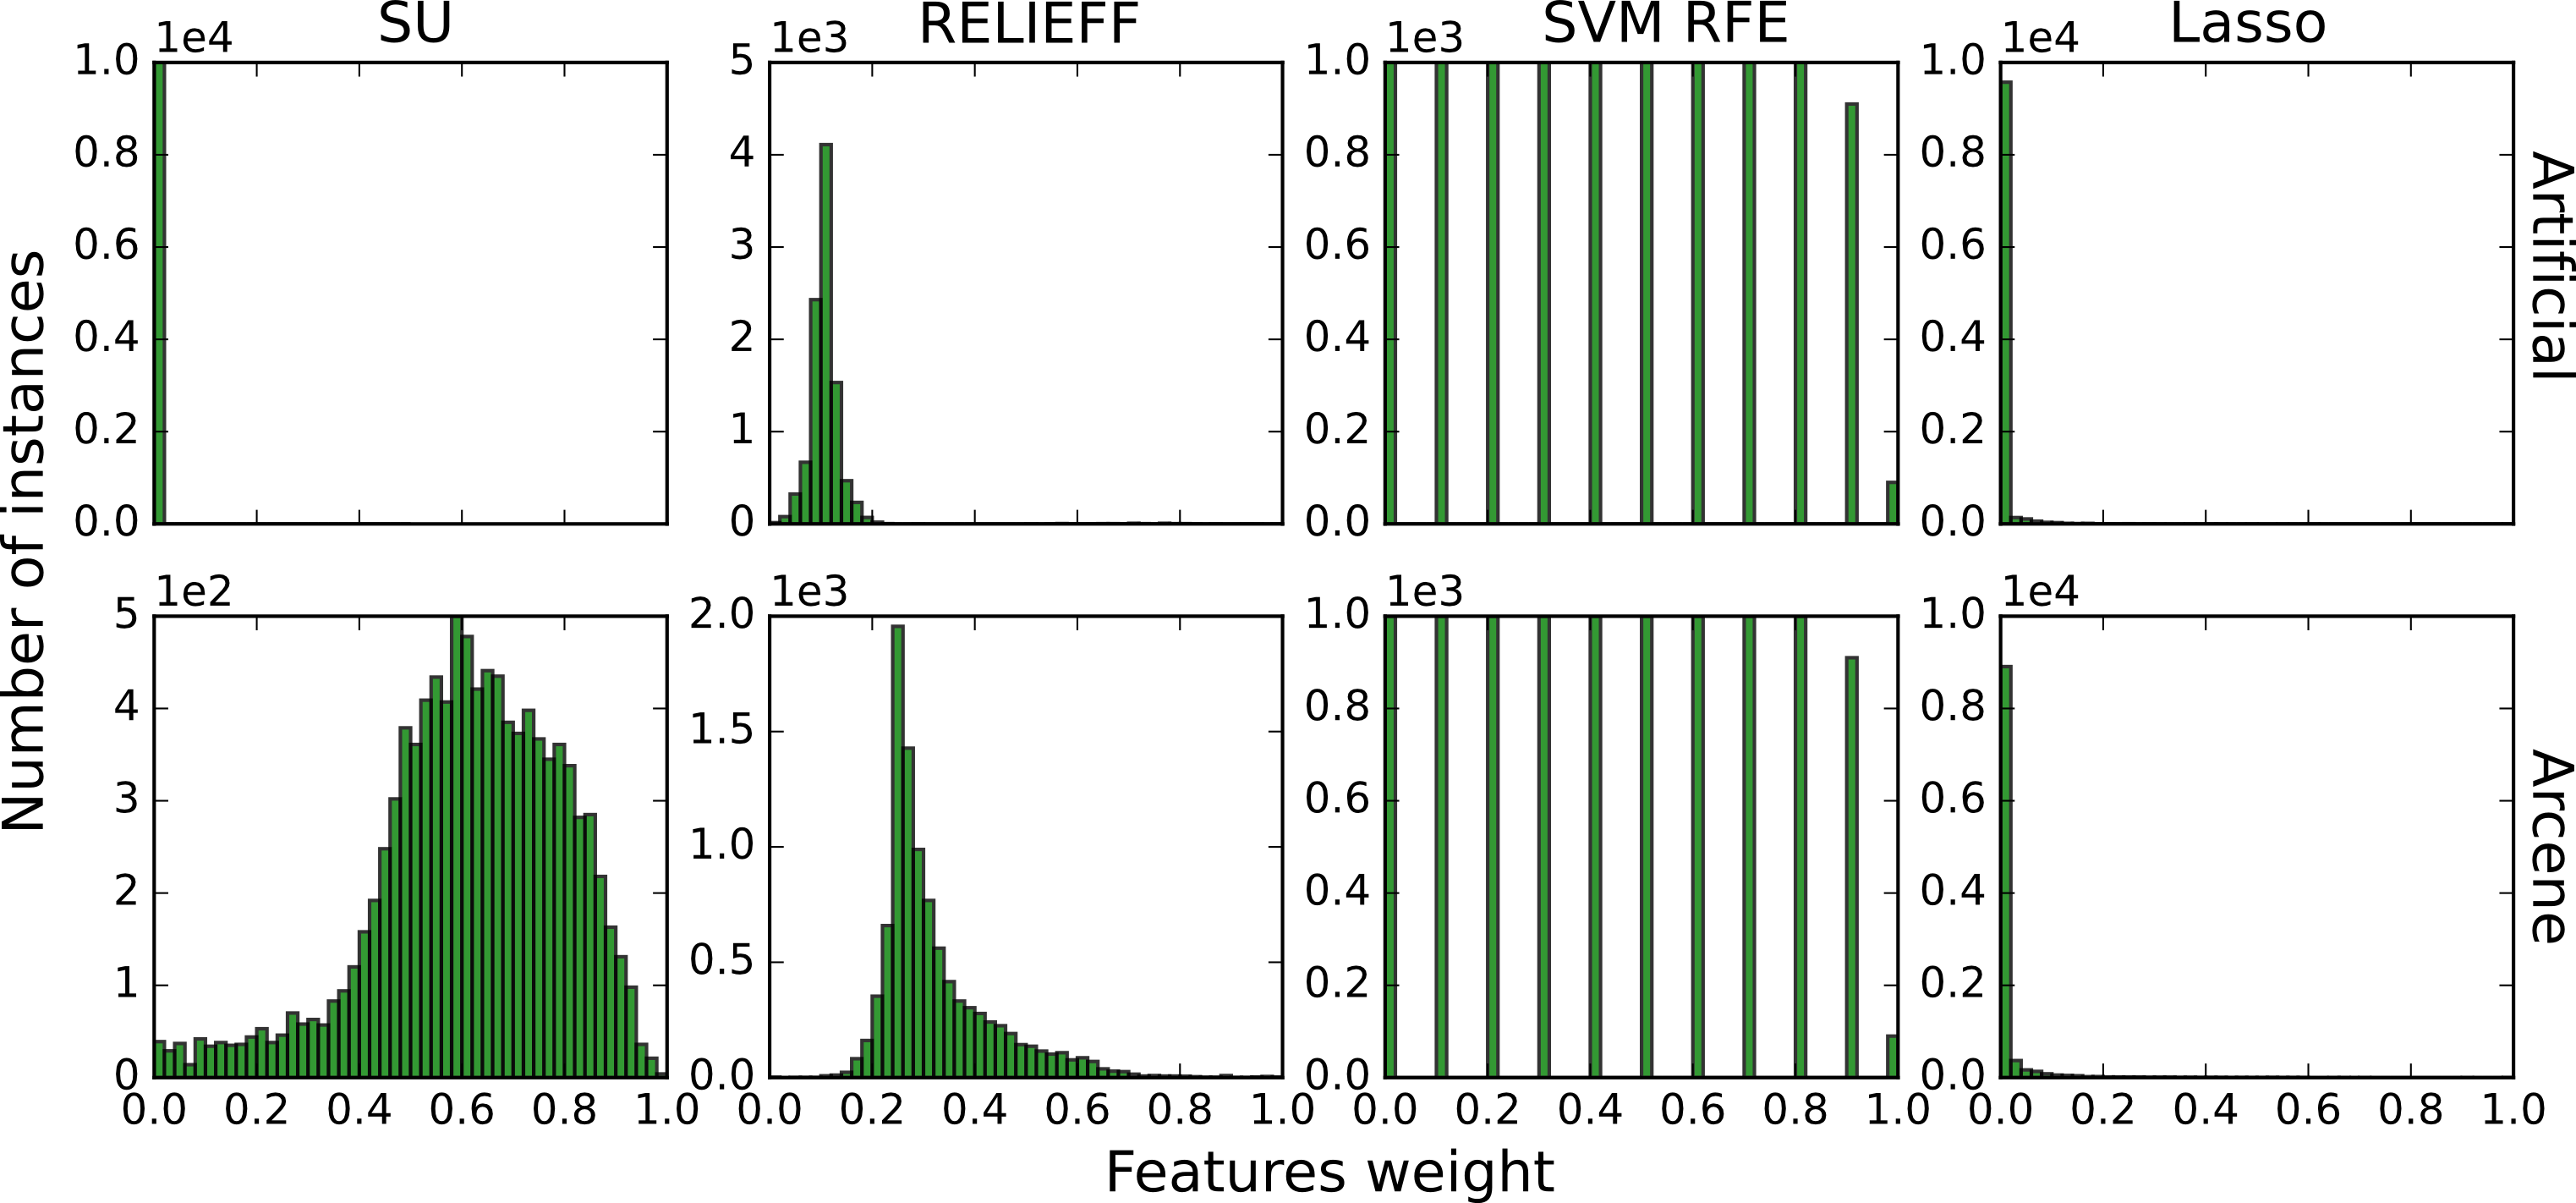
\includegraphics[width=\textwidth]{images/feature_weights_hist_arcene_artificial.png}
  \caption{The histograms of the feature weights for all used feature selectors on the arcene and artificial dataset.}
  \label{fig:feature_weights_hist_arcene_artificial}
\end{figure}

In figure \ref{fig:feature_weights_hist_arcene_artificial} the histograms of the features weight can be seen for the arcene and the artificial dataset. The histograms for all datasets can be seen in the appendix \ref{apd:plots} in figure \ref{fig:feature_weights_hist}.
It is observable that the distribution of the feature weights have similar shapes on each dataset for RELIEFF, SVM RFE, Lasso logistic regression. In addition the distributions are centered around the same area. RELIEFF and Lasso seem to always have a strong peak. Lasso even stronger than RELIEFF, which is an effect of the sparsity of Lasso. On the other hand SU varies a lot between the different datasets and does not seem to have a consistent shape. For some datasets like the artificial dataset SU mainly outputs one value for all features. On others like arcene it is greatly distributed. 

\subsubsection{Results for the artificial dataset}
\begin{figure}
  \centering 
  \begin{subfigure}[b]{0.48\textwidth}
      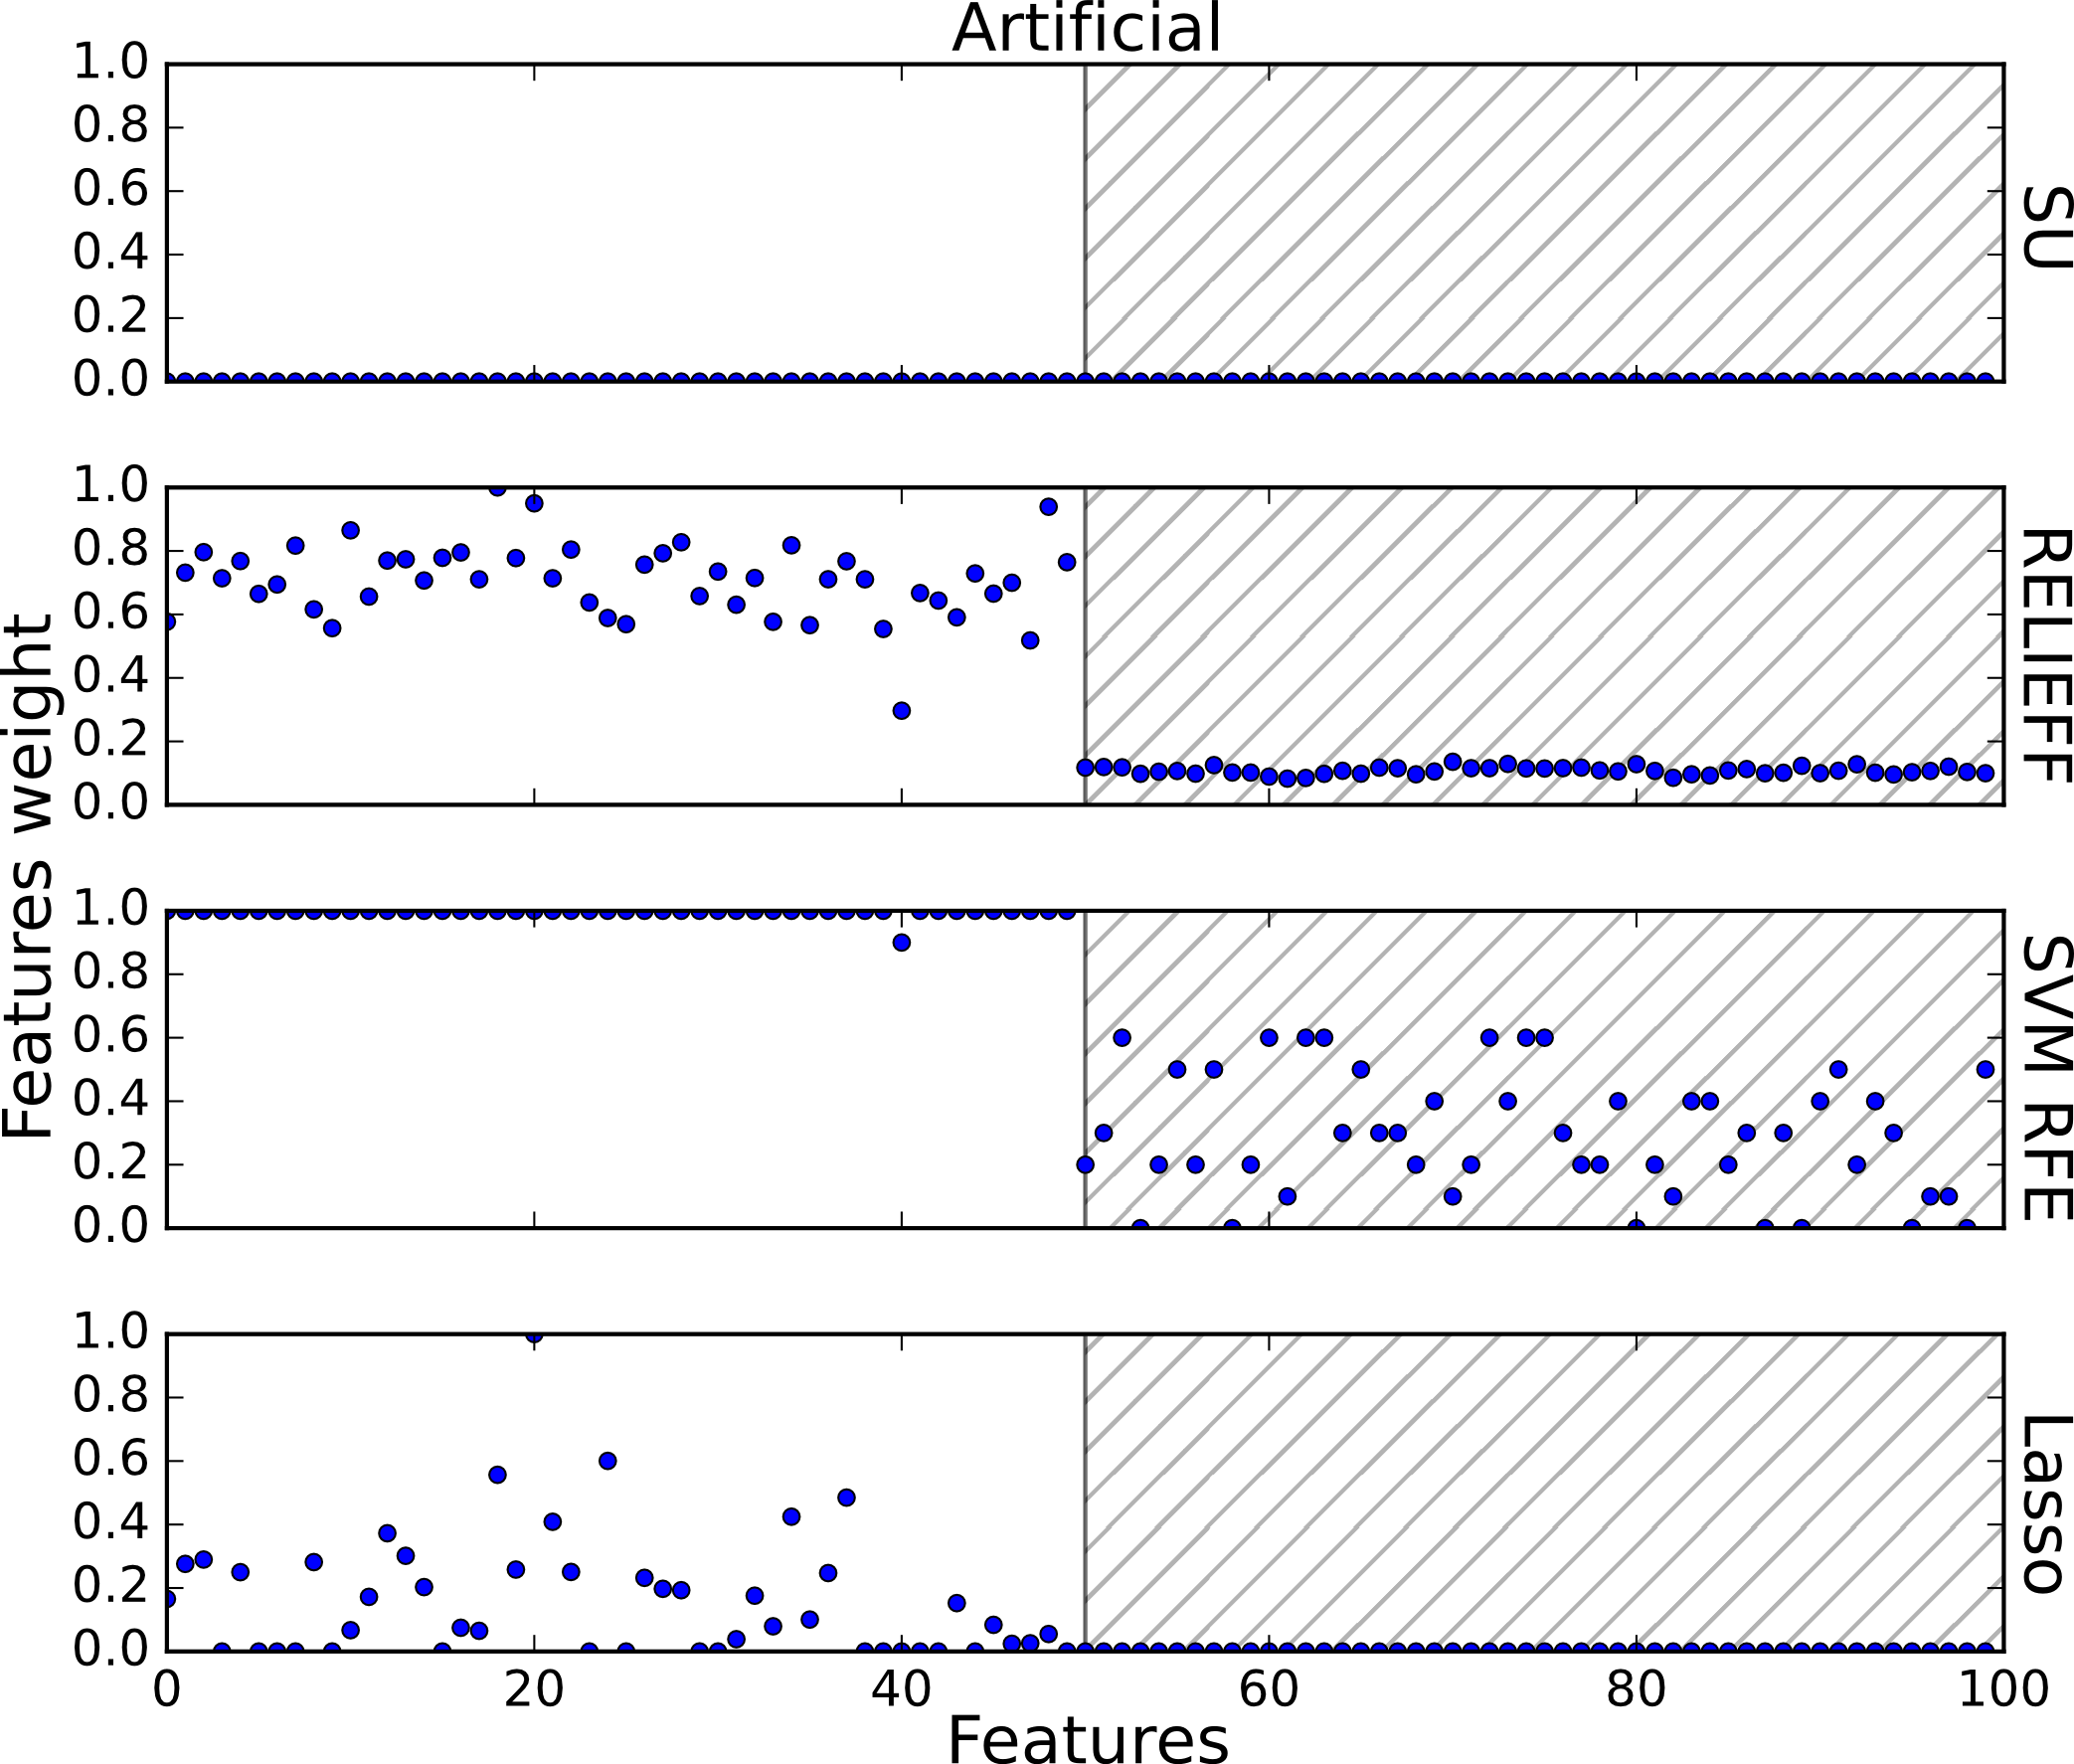
\includegraphics[width=\textwidth]{images/feature_weights_plot_artificial_only_features_bw.png}
      \caption{Features weights for the significant features.}
      \label{fig:feature_weights_plot_artificial_only_features}
  \end{subfigure}
  ~
  \begin{subfigure}[b]{0.48\textwidth}
    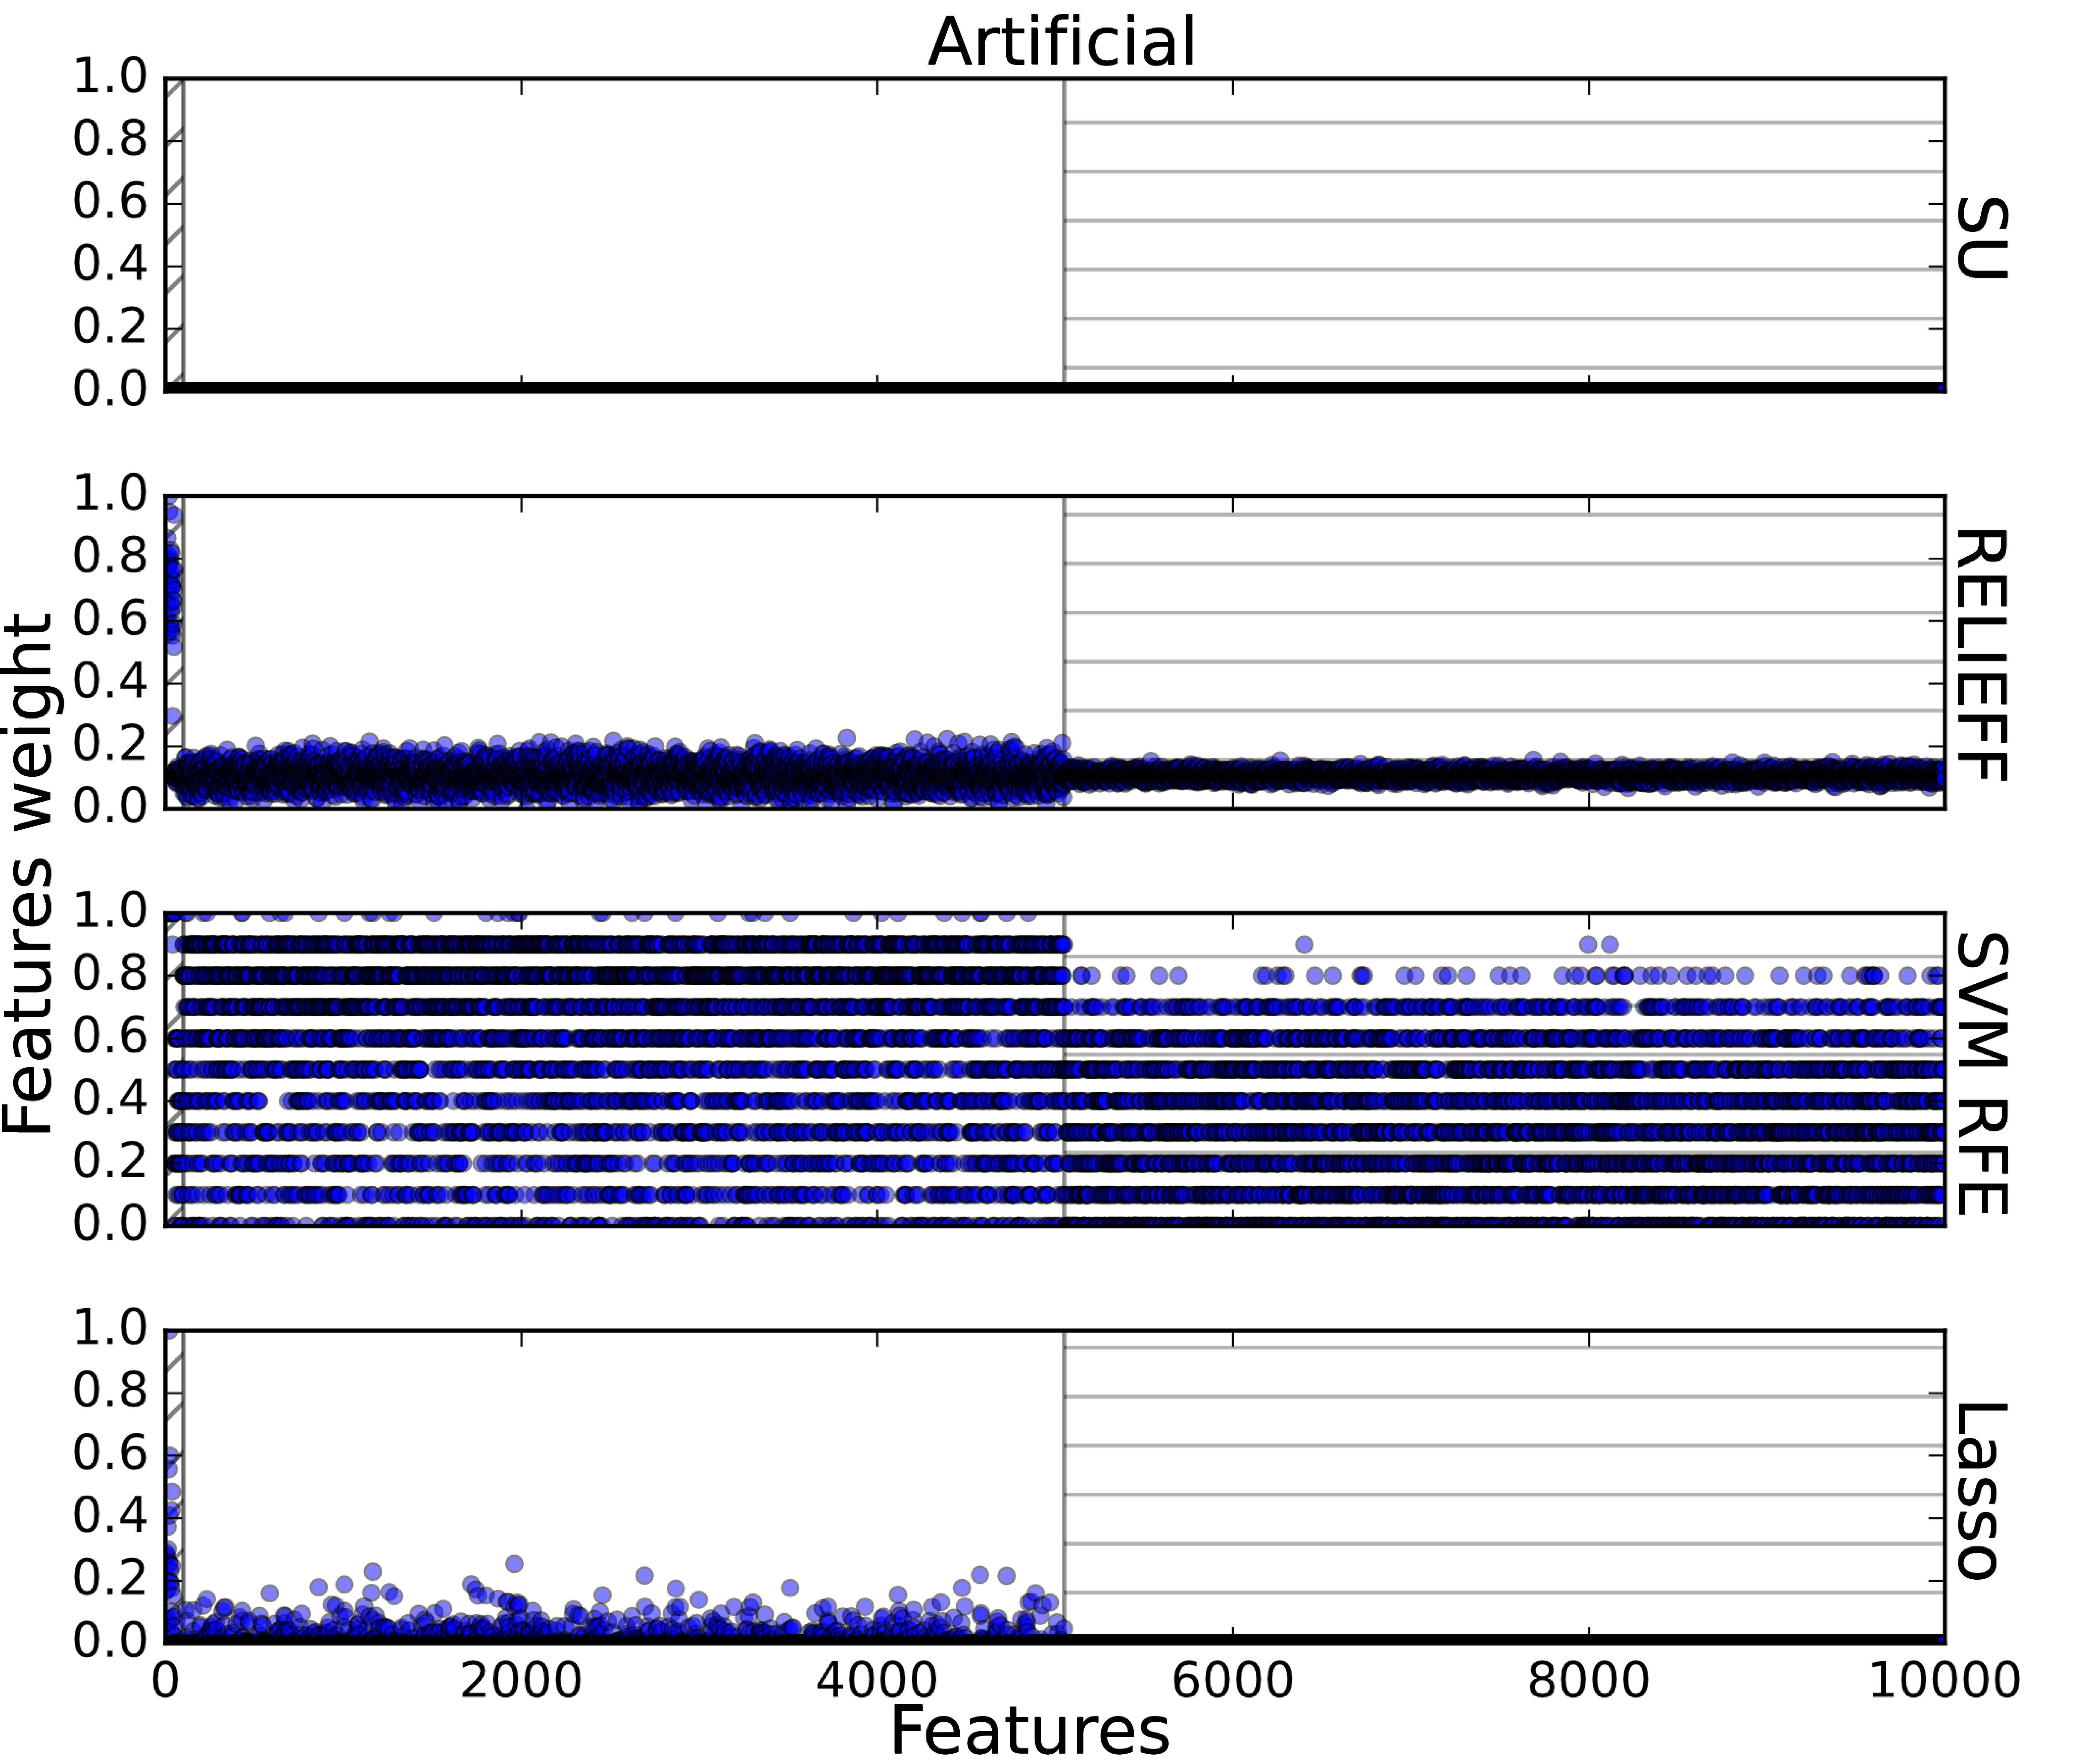
\includegraphics[width=\textwidth]{images/feature_weights_plot_artificial_all_bw.png}
      \caption{Features weights for all features.}
      \label{fig:feature_weights_plot_artificial_all}
  \end{subfigure}

  \caption{The features weights once for only the significant features and once for all features. In figure \ref{fig:feature_weights_plot_artificial_only_features} in the white area are the significant multivariate features and in the diagonal hatched area are the significant univariate features. In figure \ref{fig:feature_weights_plot_artificial_all} in the diagonal hatched area are all significant features, in the white area are the fake multivariate features and in the horizontal hatched area are the fake univariate features. }
  \label{fig:feature_weights_plot_artificial}
\end{figure}
The weights of the features can be seen in figure \ref{fig:feature_weights_plot_artificial}.
All feature selectors achieve similar results for the artificial dataset except for SU. SU ranks all features with a zero weight, making it not better than a random feature selection on this dataset. On the contrary the other feature selectors recognize parts of the inherent structure of the data. The univariate features are in general ranked lower than the multivariate features. There seems to be no difference in weighting between the significant und fake univariate features. However the significant multivariate features are ranked significantly higher than the fake multivariate features. As a consequence only multivariate features are selected. The reason why the feature selectors weight the significant univariate features this low is that the univariate features do not contribute significantly to the classification. If only the significant multivariate features are used with classification function used to generate the labels, an accuracy of $0.98$ is obtained. On the other hand using only the significant univariate features the accuracy drops to $0.52$. Therefore a feature which correlates with other significant features has significantly more impact on the classification of a data point than a uniform feature.

Furthermore, the feature selectors are evaluated with respect to how many significant features they capture in the $100$ highest weighted features. RELIEFF achieves the highest precision of $0.5$, SVM RFE achieves $0.48$, then Lasso with $0.24$ and SU with $0$.

\subsubsection{Different combinations of feature selectors}
The presented ensemble methods are used with all possible combinations of feature selectors. For each combination, the average across subsamples  is taken, and the error bar corresponds to the mean of the variance across subsamples of each ensemble method and each dataset. While the accuracy does not change considerably with the different combinations, see figure \ref{fig:combination_accuracy}, the robustness is heavily affected by the presence or absence of the feature selector Lasso as presented in the figure \ref{fig:combination_robustness}. This is due to the low robustness of the feature selector Lasso itself. On the opposite SU and RELIEFF being quite robust, their combination, with or without SVM RFE, are the most robust.  

\begin{figure}
\centering
\begin{subfigure}{.5\textwidth}
  \centering
  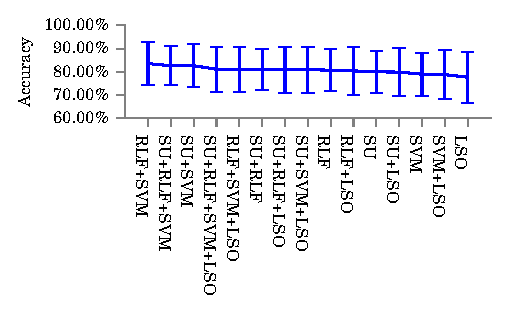
\includegraphics[width=1.07\textwidth]{images/Accuracy_of_the_different_combinations.pdf}
  \caption{Accuracy}
  \label{fig:combination_accuracy}
\end{subfigure}%
\begin{subfigure}{.5\textwidth}
  \centering
  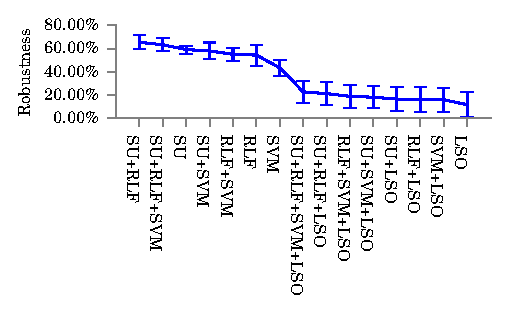
\includegraphics[width=1.07\textwidth]{images/Robustness_of_the_different_combinations.pdf}
  \caption{Robustness}
  \label{fig:combination_robustness}
\end{subfigure}
\caption{Results for the different combination of feature selectors. RLF and LSO corresponds respectively to RELIEFF and Lasso.}
\label{fig:combination_results}
\end{figure}

\subsubsection{Ensemble methods in comparison to single feature selection}

To compare the different feature selection methods in relation of robustness and accuracy, the single feature selection and the three ensemble methods achieving the best results are plotted with accuracy against stability. For the stability the Jaccard index with $1\%$ of the features is used. For the accuracy the all classifiers described in \ref{sec:experiments} are reused. For each feature selection method the standard deviation for the accuracy and the stability on the different subsets are plotted. The results for the different classifiers are similar. In figure \ref{fig:boxplot_svm} the results for the C-SVM classifier can be observed. The other results can be seen in the appendix \ref{apd:plots} in figure \ref{fig:boxplots}.
As can be seen in figure \ref{fig:boxplot_svm} the ensemble methods achieve good results on each dataset. While single feature selection methods achieve better results in terms of accuracy and robustness on some datasets, they fail on others. However the ensemble methods keep their performance for each dataset. On the arcene dataset they even achieve better results than any single feature selector. On the artificial dataset all classifiers achieve bette results with feature selection than without. For the other datasets the C-SVM classifier without feature selection achieve better results except of colon where similar results are achieved. Furthermore the random feature selection method does also achieve good results in terms of accuracy on the datasets colon, arcene and gisette.

\begin{figure}[H]
  \centering
    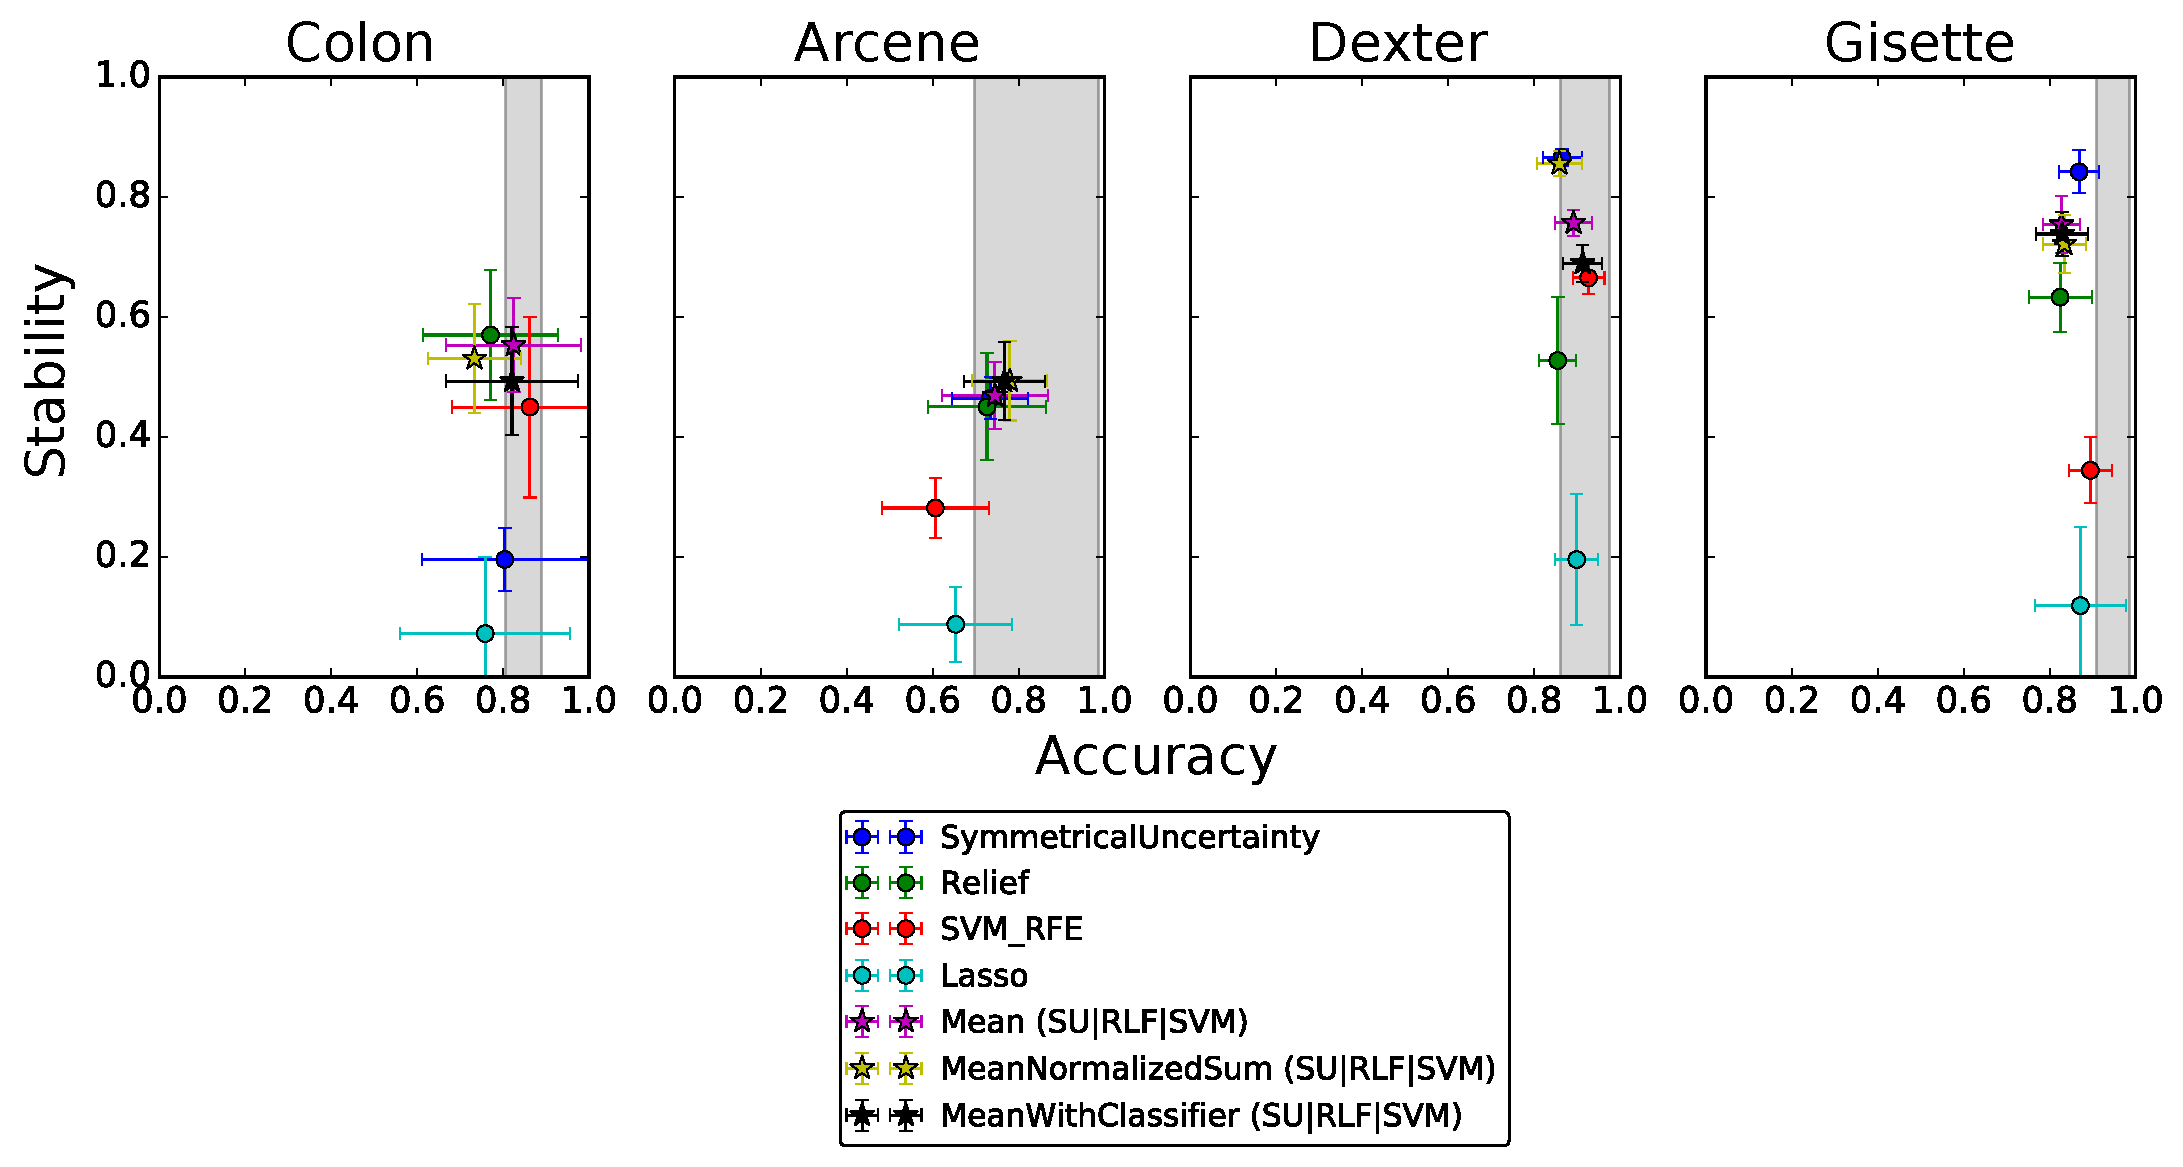
\includegraphics[width=\textwidth]{images/boxplot_svm.pdf}
  \caption{The different ensemble methods compared with single feature selectors in comparison of stability and accuracy.
  The gray area is the accuracy when using all features.}
  \label{fig:boxplot_svm}
\end{figure}

\section{Discussion}
This work shows that ensemble methods can keep up with results of single feature selectors and are even superior to the tested feature selectors in terms of generality over different datasets. Further knowledge about the weakness and strength of certain feature selectors can exploited to create good combinations of feature selectors. For the future it has to be tested if the ensemble methods in this work show similar performance on other datasets.

\vskip 0.2in
\bibliography{references}

\newpage

\appendix
\label{appendix}
\section{Python libraries}
\label{apd:libraries}
For the feature selection methods SU and RELIEFF the scikit-feature library \citep{Li-etal16} is used.
For C-SVM, RFE, Lasso logistic regression the scikit-sklearn library \citep{scikit-learn} is used.
\section{Additional plots}
\label{apd:plots}
\begin{figure}[h!]
  \centering
    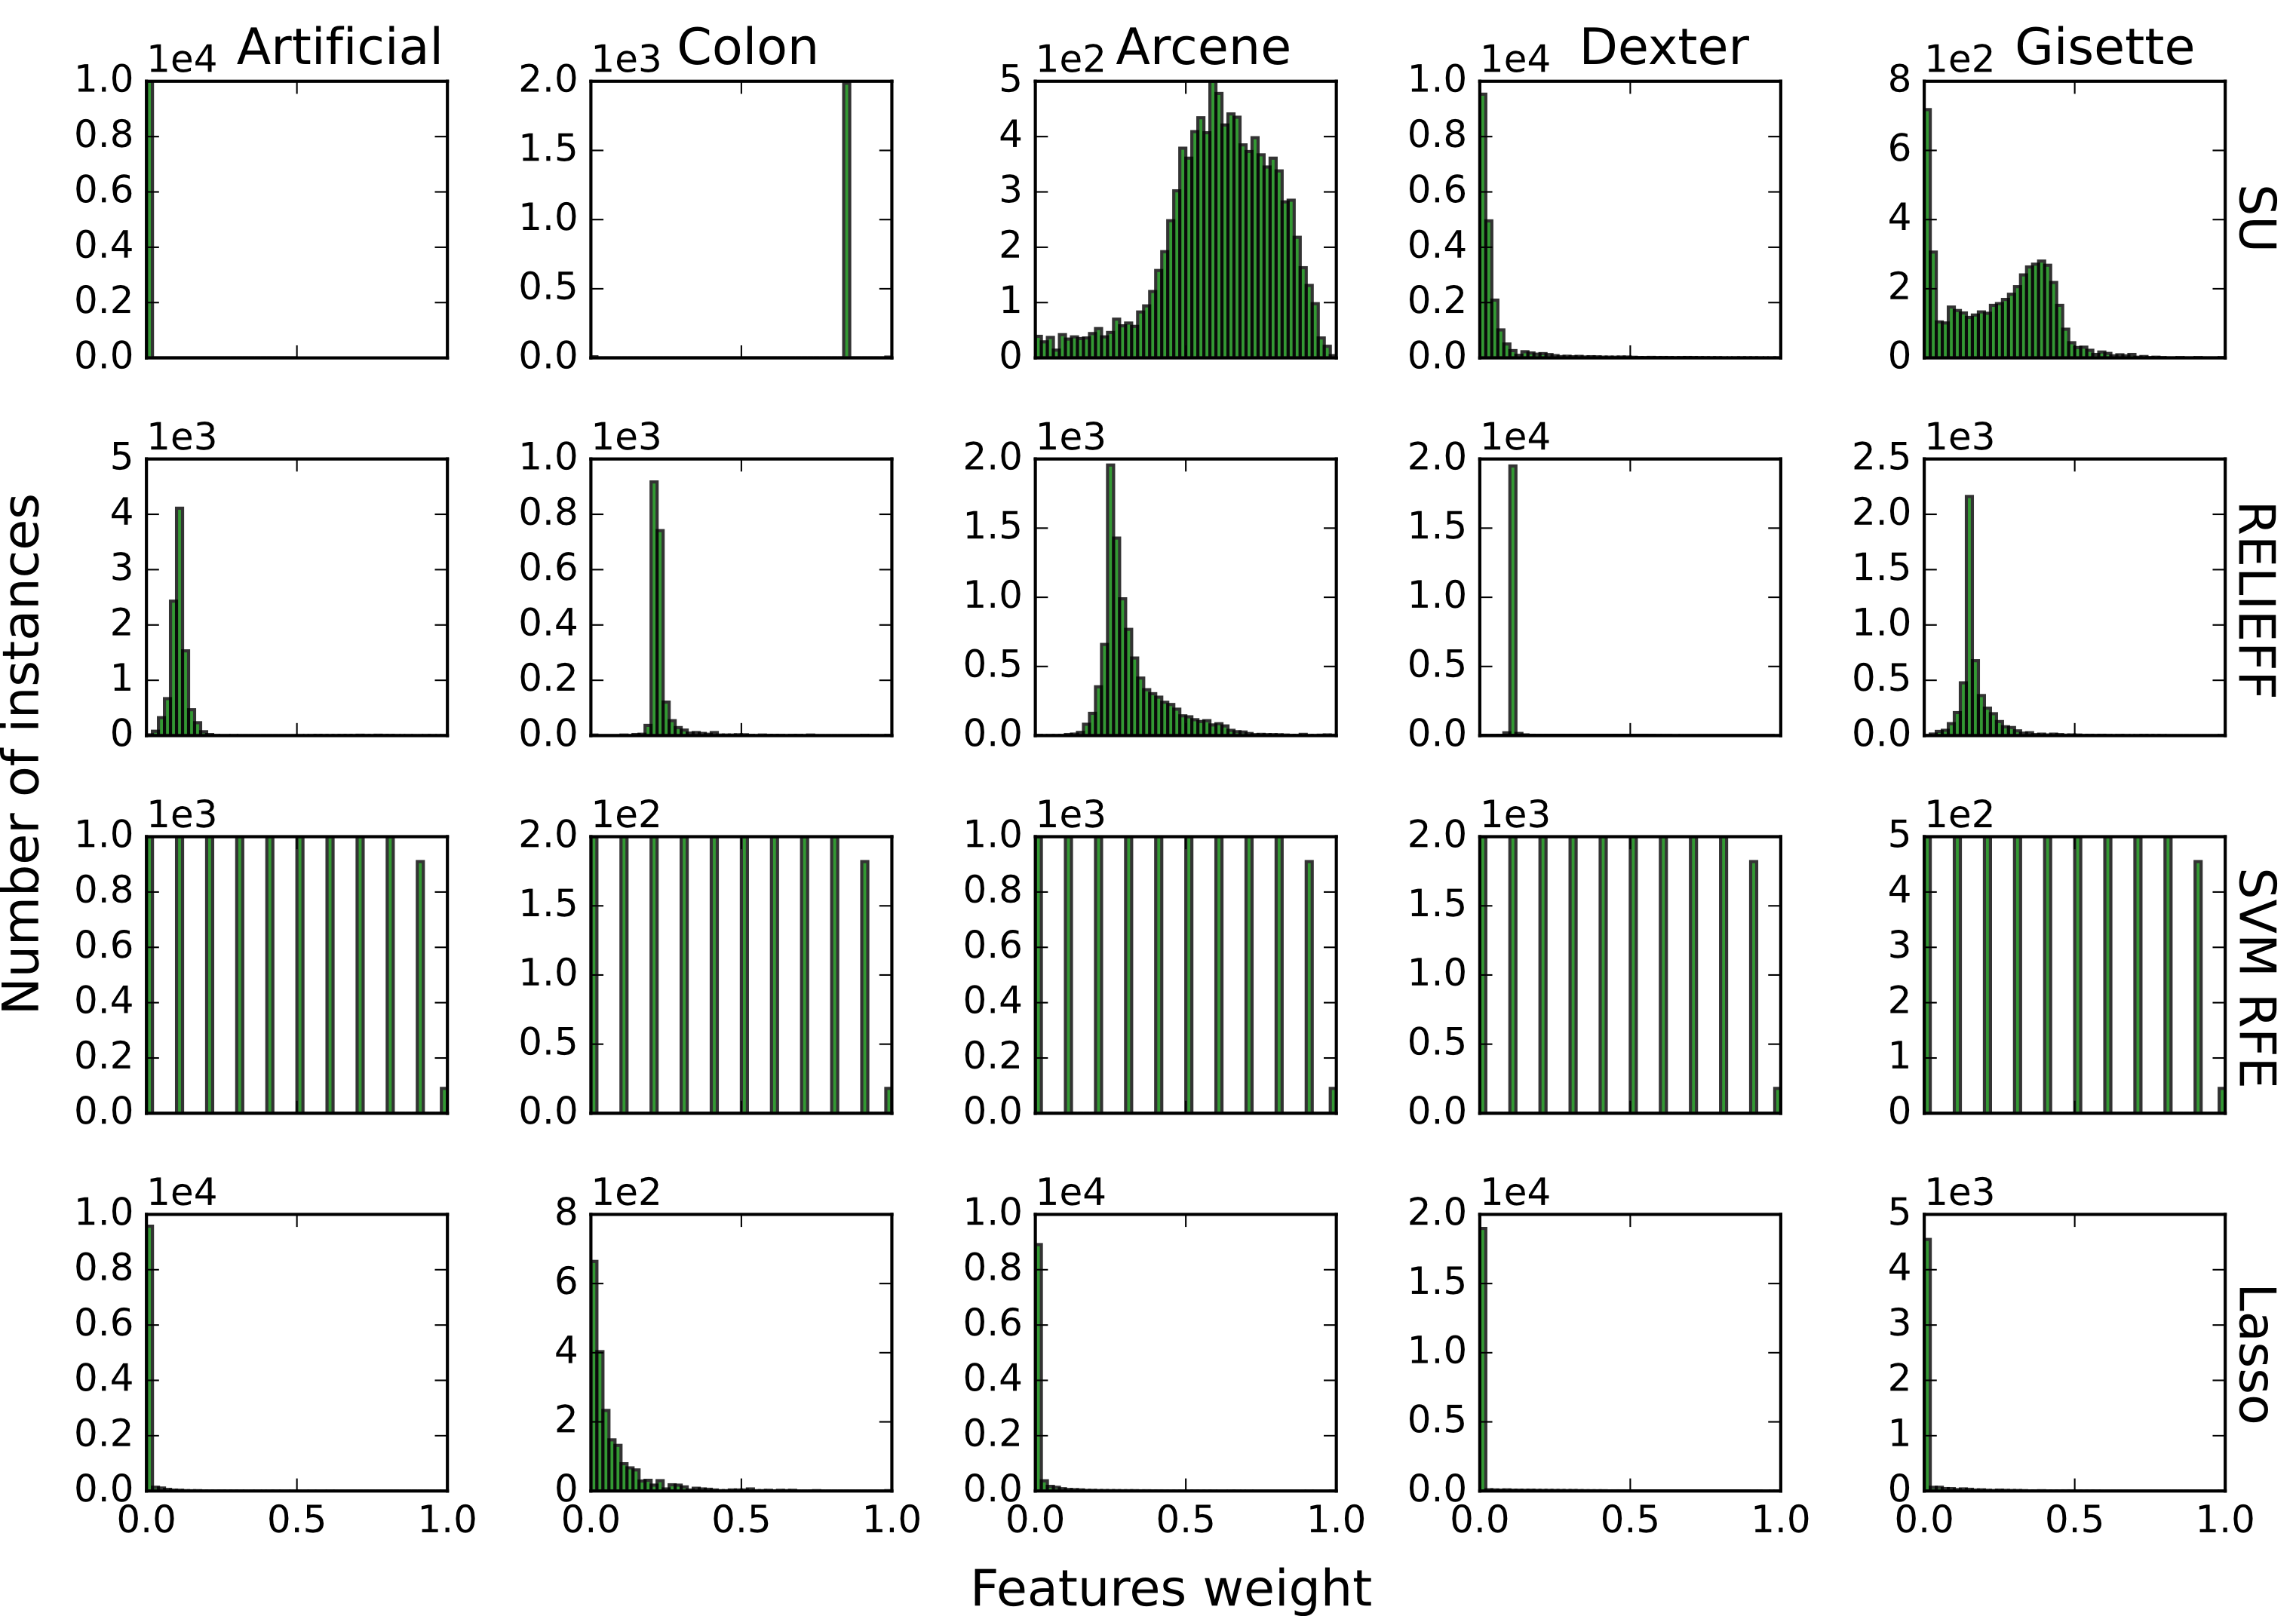
\includegraphics[width=\textwidth]{images/feature_weights_hist.png}
  \caption{The histogram of the feature weights for all feature selectors used for all datasets used.}
  \label{fig:feature_weights_hist}
\end{figure}

\begin{figure}[h!]
  \centering
    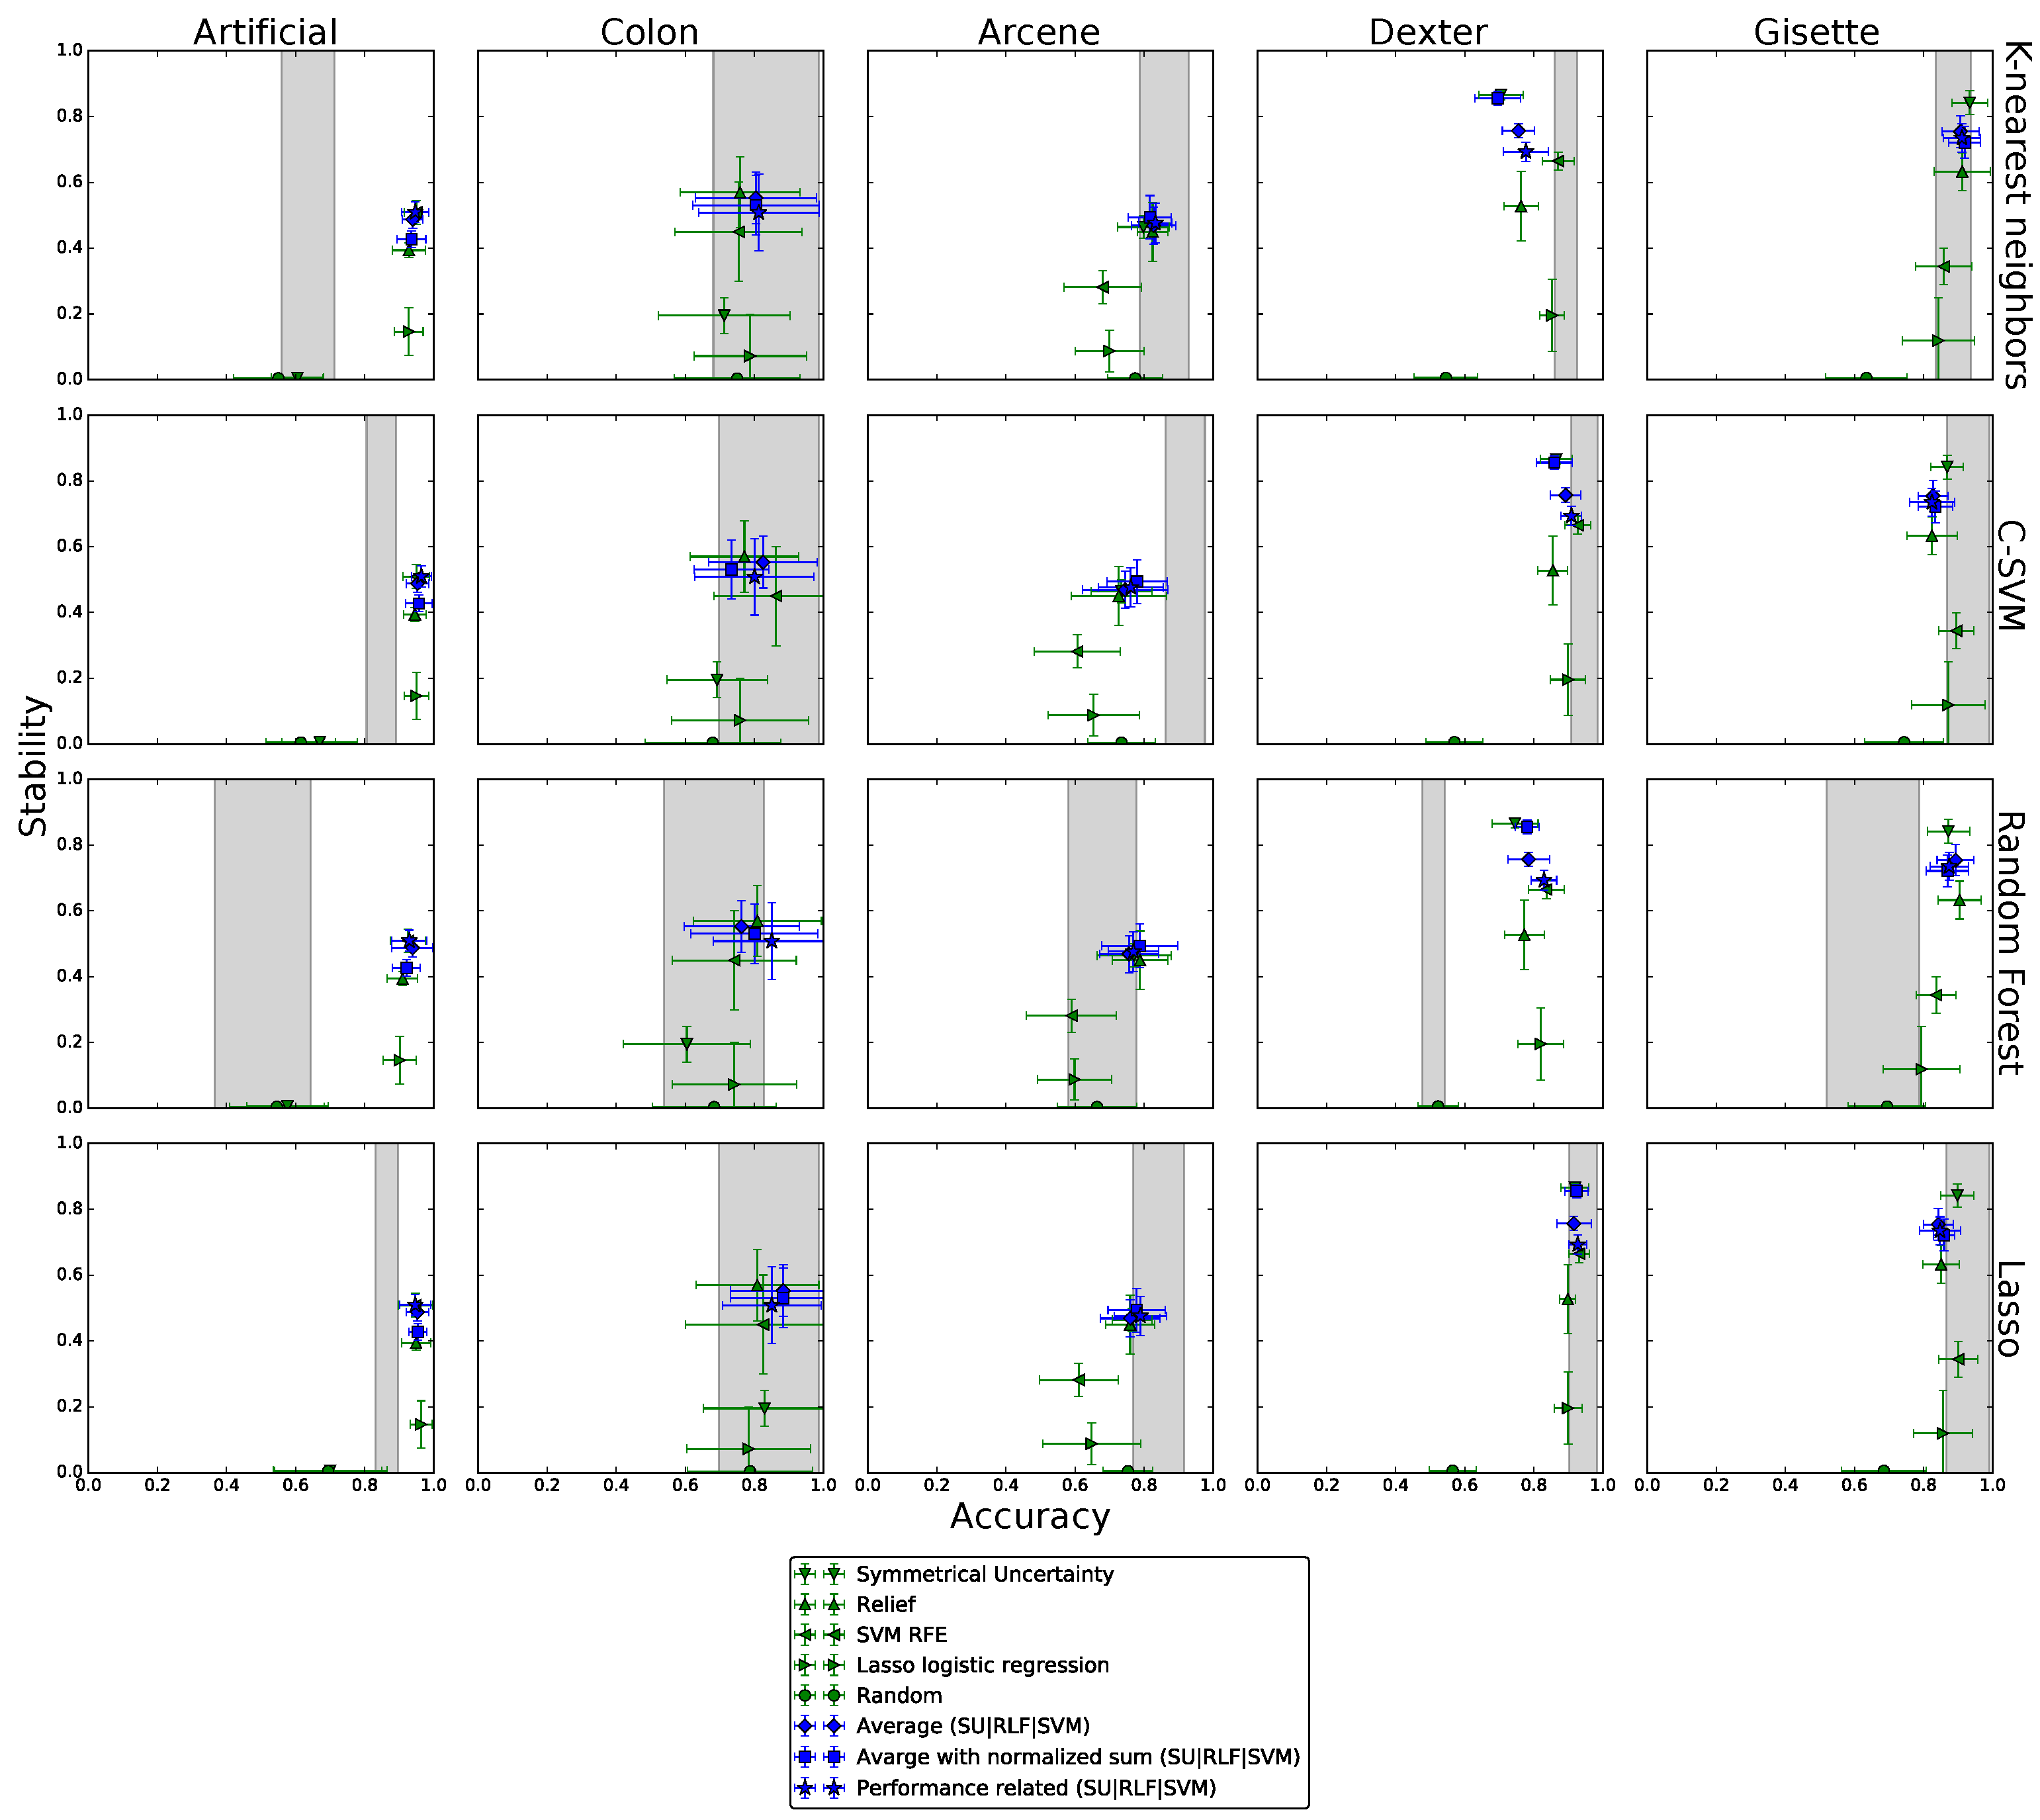
\includegraphics[width=\textwidth]{images/boxplots.pdf}
  \caption{The different ensemble methods compared with single feature selectors in comparison of stability and accuracy.
  The gray area is the accuracy when using no feature selection.}
  \label{fig:boxplots}
\end{figure}


\end{document}
